\documentclass[prb,9pt,notitlepage]{revtex4-1}
%\documentclass[a4paper,twocolumn,9pt]{article}

%\usepackage{geometry}
%\geometry{a4paper,top=2.5cm,bottom=2cm,inner=1.5cm,outer=1.5cm}

\usepackage{mwe}% just for the example content
\usepackage{color}
\usepackage{latexsym,amsmath}
\usepackage{physics}
\usepackage{listings}
\usepackage[dvipsnames]{xcolor}
\usepackage{parskip}
%\usepackage{hyperref}
%\usepackage{dblfloatfix}
%\usepackage{subfig}
\definecolor{linkcolor}{rgb}{0,0,0.65}%hyperlink
\definecolor{shadecolor}{rgb}{0.93, 0.93, 0.93}
%\usepackage[pdftex,colorlinks=true, pdfstartview=FitV, linkcolor= linkcolor, citecolor= linkcolor, urlcolor= linkcolor, hyperindex=true,hyperfigures=true]{hyperref} %hyperlink%
%\usepackage[backend=biber, sorting=ynt]{biblatex}
%\usepackage{ragged2e} % to justify caption
%\addbibresource{bibliography.bib}

\usepackage[T1]{fontenc}
\usepackage{xcolor}
\usepackage{lmodern}
\usepackage{listings}
\lstset{language=[95]Fortran,
  backgroundcolor=\color{shadecolor},
  basicstyle=\ttfamily,
  keywordstyle=\color{blue},
  commentstyle=\color{gray},
  stringstyle=\color{red},
  showstringspaces=false
  %morecomment=[l]{!\ }% Comment only with space after !
}

\usepackage{tabularx}

\usepackage{fancyhdr}
\pagestyle{fancyplain}% <- use fancyplain instead fancy
\fancyhf{}
\fancyhead[R]{\today}
\fancyhead[L]{Alessandro Lambertini}
\fancyfoot[L]{Quantum information and computing}
\fancyfoot[C]{Report 2}
\fancyfoot[R]{\thepage}

\renewcommand{\headrulewidth}{0pt}

\usepackage{float}
\usepackage{siunitx}




\begin{document}
\title{Quantum information and computing: Exercises report, week 4. \\ Multi-run script \& Automated fits }

\author{Alessandro Lambertini}


\date{\today}

\begin{abstract}
Through the exercises of this week, we try to gain confidence with some 'new' environments like gnuplot and python. Moreover, we try to build some instruments within these two environments that interact to each others and to Fortran as well. First, we have to modify the exercise 3 of week 1 in a way that allows the dimensions of the matrices to be read from a file. Second, we have to write a Python script that changes the dimensions $N$ between two values $N_{min}$ and $N_{max}$, launches the Fortran program, and stores the time needed to perform the multiplication in different files depending on the multiplication method used. Then, we plot the results for the three different methods using Gnuplot. After that, we exploit gnuplot to perform the fit of the time needed to perform the multiplication for the three methods as a function of the dimension of the matrix. Finally, we exploit the gnuplot files used before to write a python script that perform automatically the previous fit.
\end{abstract}

\maketitle

\section{Theory}
\subsection{Access to files}
Both in Fortran and in Python the way to deal with files is very straightforward.

In Fortran there is the \textit{open()} function that allows to access a file to perform some operations:
\begin{lstlisting}
  open(unit=u,file=filename)
\end{lstlisting}
where the argument \textit{unit} is an integer that represents the pointer of the file for the I/O operations.

Then, to write and read to and from the file there are two intrinsic functions called \textit{write()} and \textit{read()}
whose formal syntax is:
\begin{lstlisting}
  read ([UNIT = ]u, [FMT = ]fmt, IOSTAT = ios, ERR = err, END = s)
  write([UNIT = ]u, [FMT = ]fmt, IOSTAT = ios, ERR = err, END = s)
\end{lstlisting}
where the argument \textit{FMT} is the format specifier.
Finally there is the \textit{close(unit)} function to to stop the operations performed on the file.

In Python instead, a name is assigned to the file and operations are carried out through \textit{methods}, an example could be:

\begin{lstlisting}
  f = open("filename.txt","w")
  f.write(...)
  f.close()
\end{lstlisting}
Where the file \textit{filename.txt} is opened to be written and werefer to it with the name \textit{f}. We write something on file with the method \textit{write()} and then we close it with the method \textit{close}.

\subsection{scripts}
The distinction between a normal program and a script is not clear-cut, but generally the following characteristics can be identified in scripts:
\begin{itemize}
  \item relatively low complexity;
  \item use of an interpreted language;
  \item a certain linearity (a script can also accept input from the user, but usually different inputs do not substantially change the structure of the block diagram that describes the behavior of the script);
  \item lack of its own graphical interface;
  \item recall of other programs to perform more sophisticated operations.
\end{itemize}
In particular we will recall from Python scripts Fortran an Gnuplot program to be executed with a set-up specified by the scipt.

\subsection{Gnuplot}
Gnuplot is a program for exploring data graphically. Its purpose is to generate plots and graphs from data or functions. It can produce highly polished graphs, suitable for publication, or simple throw-away graphs when you’re merely playing with an idea.
The most important command in Gnuplot is \textit{plot}. This command is used to plot functions and data and has a lot of options and subcommand to control the appearance of the graphs. To plot different objects in the same graph they have to be under the same \textit{plot} command, separated by a comma. If a plot of a function and a dataset contained in a file is needed, the basic syntax is:
\lstset{language=Gnuplot,
  backgroundcolor=\color{shadecolor},
  basicstyle=\ttfamily,
  keywordstyle=\color{black},
  commentstyle=\color{gray},
  stringstyle=\color{black},
  showstringspaces=false
  %morecomment=[l]{!\ }% Comment only with space after !
}
\begin{lstlisting}
  plot "filename", f(x)
\end{lstlisting}

To perform the fit of a function $f(x)$, defined by the user, over a dataset it is needed the \textit{fit} command, which exploit the nonlinear least-squares (NLLS) Marquardt-Levenberg algorithm. The general syntax for this command is:
\begin{lstlisting}
fit {[xrange] {[yrange]}} <function> '<datafile>' {datafile-modifiers}
    via '<parameter file>' | <var1>{,<var2>,...}
\end{lstlisting}
Where command between curly brackets are optional.

\section{Code development}
The first thing required by the exercises is to modify the exercise 3 of week 1 so that the dimension of the matrix, in this case a square matrix, is read from a file. Initially, I implemented a change in the subroutine that initializes the matrices, but it turns out that this is not the best approach because it requires a lot of changes in all the other subroutine used in the program and in the structure of the program itself. Therefore, I have modified the program with three simple lines of code:

\lstset{language=[95]Fortran,
  backgroundcolor=\color{shadecolor},
  basicstyle=\ttfamily,
  keywordstyle=\color{blue},
  commentstyle=\color{gray},
  stringstyle=\color{red},
  showstringspaces=false
  %morecomment=[l]{!\ }% Comment only with space after !
}

\begin{lstlisting}
  open(unit=1, file='dim.txt')
  read(1,*) dim_m1(1),dim_m1(2),dim_m2(1),dim_m2(2)
  close(1)
\end{lstlisting}
Where we open the file \textit{dim.txt} read from it the first four items, which must be integers, and assign them to the elements of two one-dimensional arrays with two entries each.

Then, we are required to write a Python script that changes the value of the dimensions of the matrix, launches the Fortran program and store the results in different files depending on the method used for the multiplication. To do so, i implemented the following Python script:
\lstset{
language=Python,
basicstyle=\ttfamily,
keywordstyle=\color{blue},
emph={MyClass,__init__},
emphstyle=\color{red},
stringstyle=\color{green!50!black},
showstringspaces=false
}
\begin{lstlisting}
import os

N_min = input('Enter N_min:')
N_min = int(N_min)
N_max = input('Enter N_max:')
N_max = int(N_max)
step = input('Enter step:')
step = int(step)

for i in range(N_min,N_max,step):
  f= open("dim.txt","w")
  f.write('%d,%d,%d,%d' % (i,i,i,i))
  f.close()
  os.system("./ex04")
  print(i)
\end{lstlisting}

This script, named \textit{cng\_dim\_sv\_rn.py}, exploit the module 'os' to call the Fortran program. Moreover, I implemented the possibility for the user to choose the range in which $N$, the dimension of the matrix, have to vary and the step between a value and the next one.
\newpage
The task of storing the results is accomplished within the Fortran program with the following idea:
\lstset{language=[95]Fortran,
  backgroundcolor=\color{shadecolor},
  basicstyle=\ttfamily,
  keywordstyle=\color{blue},
  commentstyle=\color{gray},
  stringstyle=\color{red},
  showstringspaces=false
  %morecomment=[l]{!\ }% Comment only with space after !
}

\begin{lstlisting}
  call cpu_time(start)

  call mat_mul_loop#(...)  !subroutine to perform the multiplication
                           !with a specific method

  call cpu_time(finish)

  open(unit=##,file='time_loop#.csv',Access = 'append') !open the file for that
                                                        !specific loop

  write(#,'(I0,A,F0.15)')  dim_m1(1),',', finish-start  !write the dimension
                                                        !and the the time needed
                                                        !to complete the task
  close(##)  !close the file
\end{lstlisting}
These method is used to store the results of all the three methods present in the program. These are all the changes implemented in the Fortran program which is named \textit{ex\_04.f90}.
Moreover, we are required to plot, using Gnuplot, the results for the different multiplication methods and then to perform the fit over the biggest possible difference between $N_{min}$ and $N_{max}$.

In order to do this, I wrote two different Gnuplot files . The first one implement the fit of the data with a power-law $f(x)=ax^b$, as expected from theory. This is the simple syntax used:
\lstset{language=Gnuplot,
  backgroundcolor=\color{shadecolor},
  basicstyle=\ttfamily,
  keywordstyle=\color{black},
  commentstyle=\color{gray},
  stringstyle=\color{black},
  showstringspaces=false
  %morecomment=[l]{!\ }% Comment only with space after !
}
\begin{lstlisting}
  set datafile separator ','
  set grid xtics mxtics ytics mytics back
  set title 'Fit of time_loop1.csv'
  set xlabel 'N'
  set ylabel 't'
  set key right bottom
  f(x) = a*x**b
  a=1e-8
  b=3
  fit f(x) 'time_loop1.csv' via a,b
  set label 1 'model: f(x)= a*x**b' at 200,60 font 'courier,15'
  set label 2 sprintf("a=%3.4es", a) at 200,56 font 'courier,15'
  set label 3 sprintf("b=%3.4es", b) at 200,52 font 'courier,15'
  plot 'time_loop1.csv' w p lc 'red' title 'data', f(x) title 'fitted curve'
\end{lstlisting}
The second file implement the fit with the linearized data. This is done by performing the logarithm of both x-axis data and y-axis data. In this way we expect the data to be positioned along a straight line. The simple syntax used to obtain the plot is:
\begin{lstlisting}
  set datafile separator ','
  set grid xtics mxtics ytics mytics back
  set title 'Fit of linearized time_loop2.csv'
  set xlabel 'log_{10}N'
  set ylabel 'log_{10}t'
  f(x) = a*x+b
  a=3
  b=-10
  fit f(x) 'time_loop2.csv' u (log10($1)):(log10($2)) via a,b
  set label 1 'model: f(x)= a*x+b' at 2.2,2 font 'courier,15'
  set label 2 sprintf("a=%3.4es", a) at 2.2,1.7 font 'courier,15'
  set label 3 sprintf("b=%3.4es", b) at 2.2,1.4 font 'courier,15'
  plot 'time_loop2.csv' u (log10($1)):(log10($2)) w p lc 'red' title 'data',
       f(x) title 'fitted curve'
\end{lstlisting}
Finally, we have to write a python script that perform automatically the fits implemented in the two Gnuplot files above. I implemented two python scripts very similar to each other named \textit{fit\_gnu.py} and \textit{fit\_gnu\_log.py}. Here is the second one:

\lstset{
language=Python,
basicstyle=\ttfamily,
keywordstyle=\color{blue},
emph={MyClass,__init__},
emphstyle=\color{red},
stringstyle=\color{green!50!black},
showstringspaces=false
}

\begin{lstlisting}
#######single-variable fit with gnuplot log-log version###########

import PyGnuplot as gp

###########collecting all the variable from the user##############
data_sep = input('Enter separator character:')
data = input('Enter the name of the file containing the data:')
func = input('Enter the function to fit with gnuplot syntax (f(x)=...):')
num_par = input('Enter the number of parameters:')
num_par = int(num_par)
param_name = []
param_value = []
for i in range(num_par):
  b = input('Enter the name of the parameter #'+str(i+1)+':')
  a = input('Enter the guess for the parameter #'+str(i+1)+':')
  param_value.append(a)
  param_name.append(b)



################### structure them in a gnuplot format #######################
k=' '
for i in range(num_par):
  k = k+param_name[i]+','
s = list(k)
s = s[:-1]
s = ''.join(s)

tit = input('Enter the title of the plot:')
x_label = input('Enter x label:')
y_label = input('Enter y label:')


gp.c("set datafile separator '"+data_sep+"''")
gp.c('set grid xtics mxtics ytics mytics back ')
gp.c("set title '"+tit+"'")
gp.c('set key right bottom')
gp.c('set xlabel "'+x_label+'"')
gp.c('set ylabel "'+y_label+'"')
gp.c(func)
for i in range(num_par):
  gp.c(param_name[i]+'='+param_value[i])
gp.c("fit f(x) '"+data+"' u (log10($1)):(log10($2)) via"+s)
gp.c('set label 1 "model: '+func+'" at 2.1,1.5 font "courier,15')

#for i in range(num_par):
  #gp.c('set label '+str(i+2)+'sprintf("'+param_name[i]+'=%3.4f",
  #'+param_name[i]+') at 2.1,'+str(1.3-0.2*i)+' font "courier,15"')

gp.c("plot '"+data+"' u (log10($1)):(log10($2)) w p lc 'red' title 'data',
f(x) title 'fitted curve'")
\end{lstlisting}
In this script, essentially, I reproduced the behaviour of the \textit{plot\_loop2.gnuplot} file through a Python package called \textit{PyGnuplot}. What changes is that the file with the data and the function to be fitted are given by the user through the command line but in a more natural way, without the Gnuplot commands. The only things that is missing in this script that are present in the two gnuplot files above are the three labels with the function model and the estimation of the parameters. I did not found a way to automatize the positioning of these labels. With a bit more time I will correct this problem.



\section{Results}
In \ref{fig:foobar} are reported all the six fits produced with $N$ varying from $100$ to $2000$ , three with the power-law scaling and three linearized; two for each methods of multiplication used. We obtained what we essentially expected from theory. It is evident the $O(n^3)$ scaling time structure in general for all the three algorithm, but it is also possible to appreciate the difference in the optimization between them, with the intrinsic function accomplish far better results in the long run.

All the files produced to complete the exercises are located in the folder \textit{Ex4-Lambertini-CODE}.

\begin{figure}[H]
    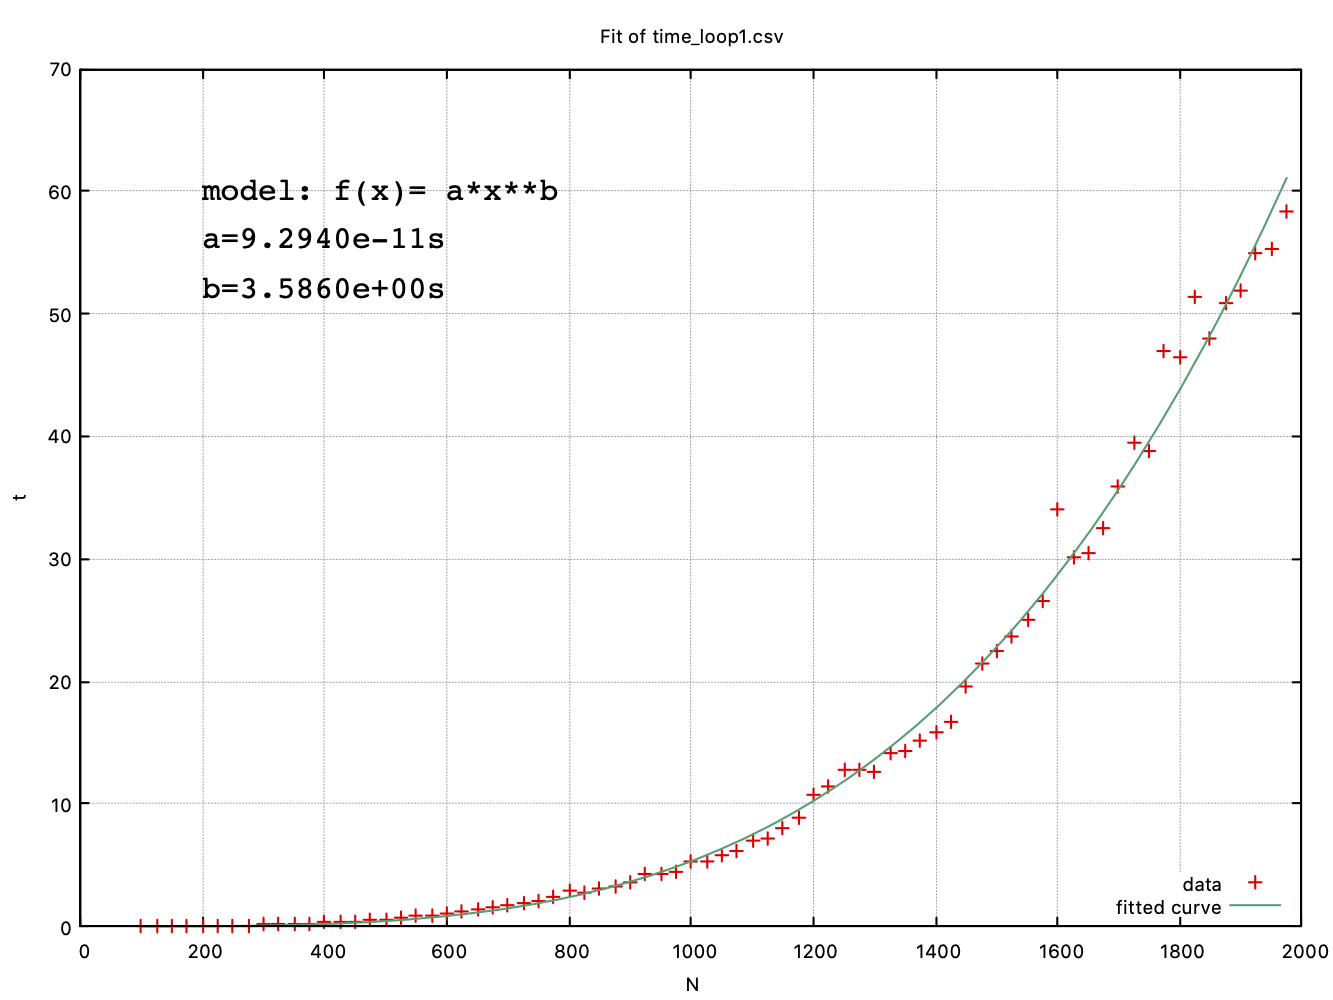
\includegraphics[width=.32\textwidth]{time_loop1}\hfill
    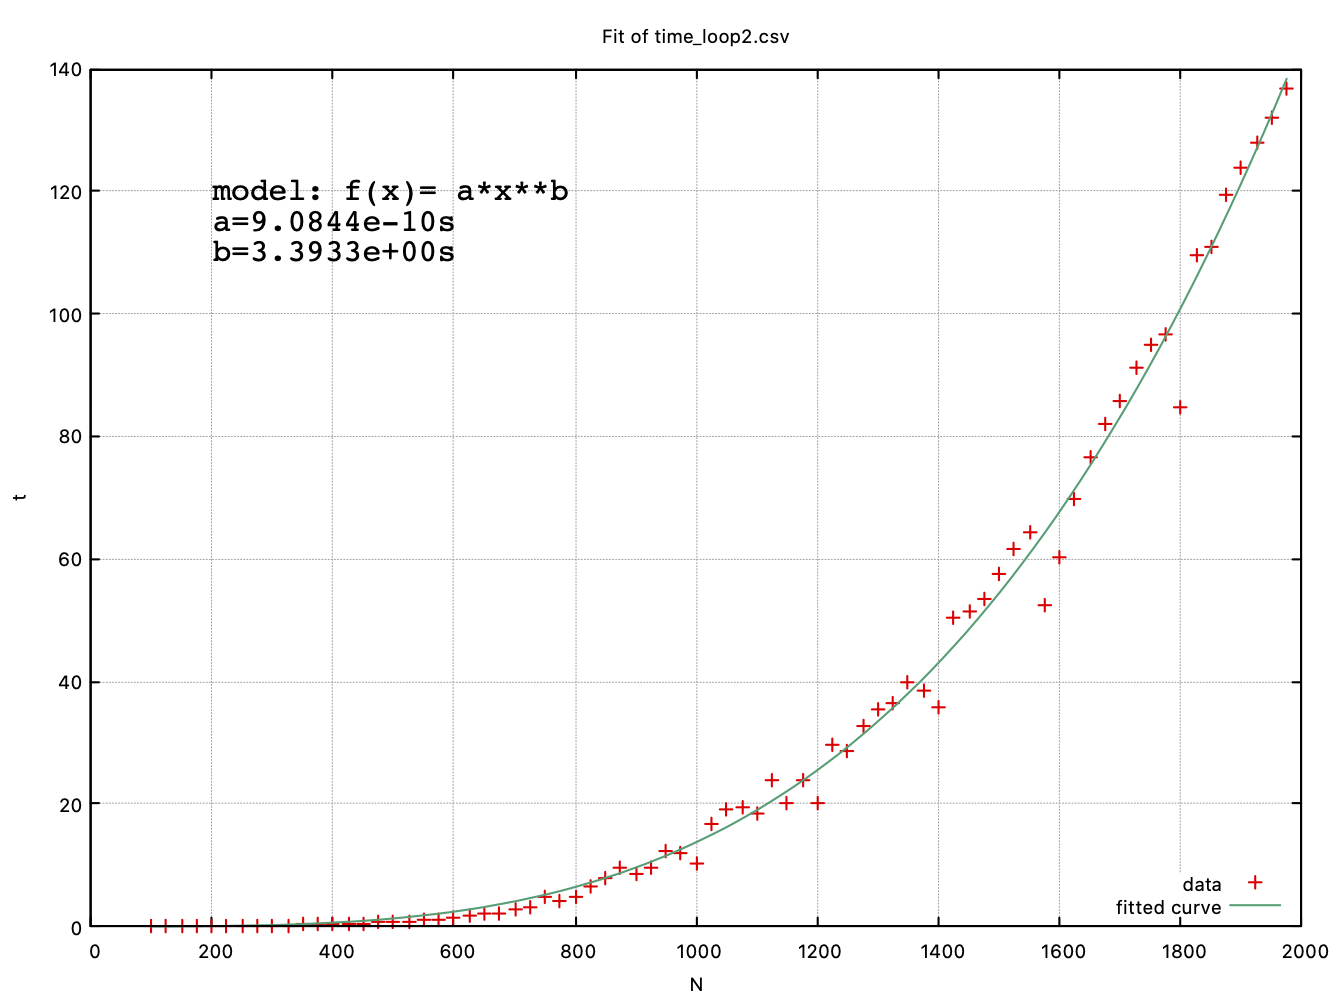
\includegraphics[width=.32\textwidth]{time_loop2}\hfill
    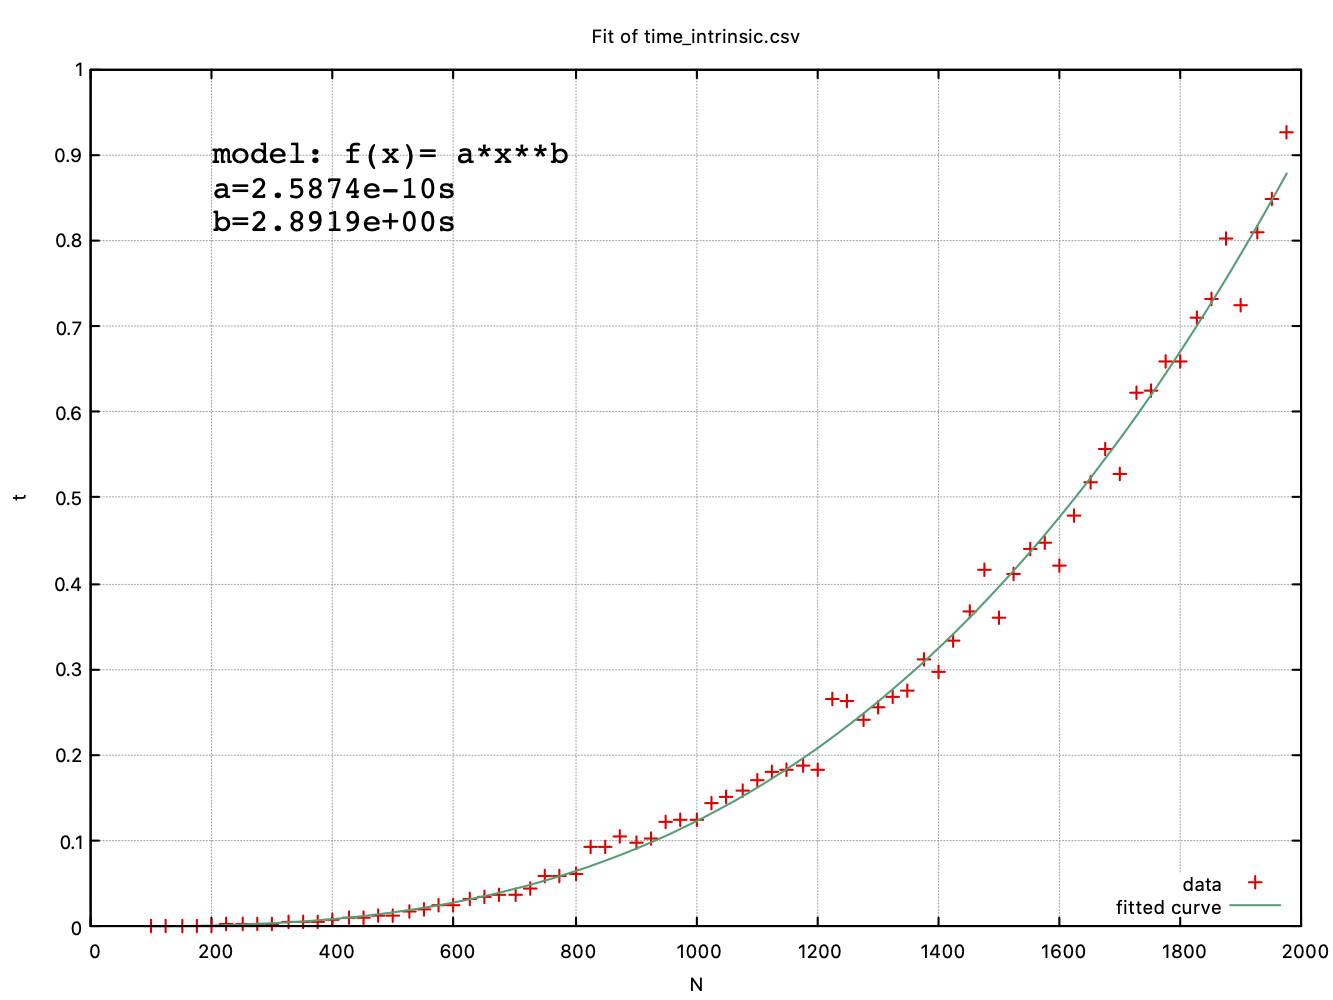
\includegraphics[width=.32\textwidth]{time_intrinsic}
    \\[\smallskipamount]
    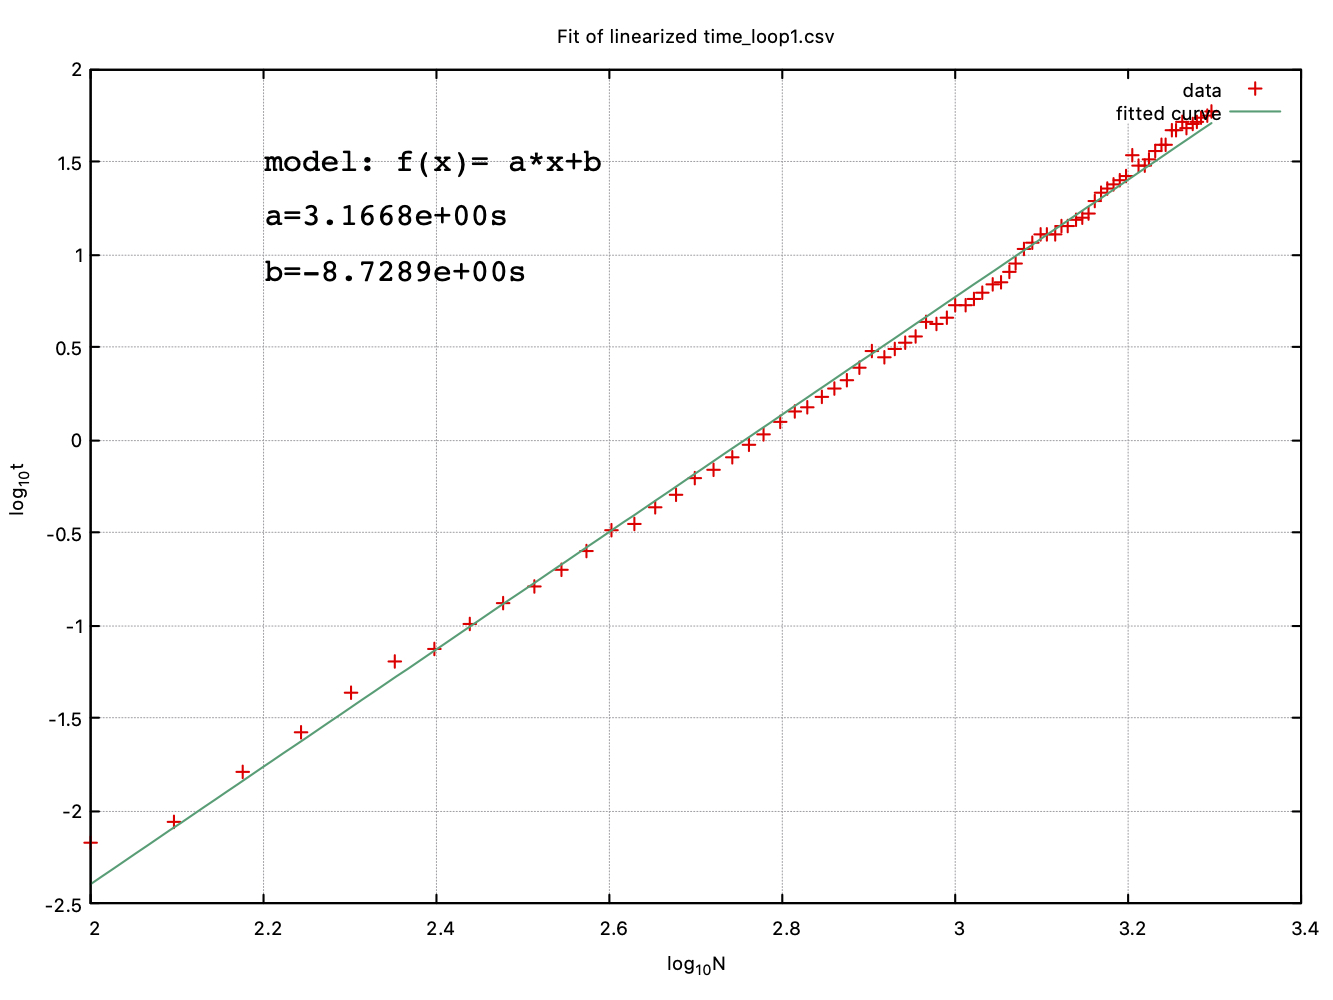
\includegraphics[width=.32\textwidth]{time_loop1_lin}\hfill
    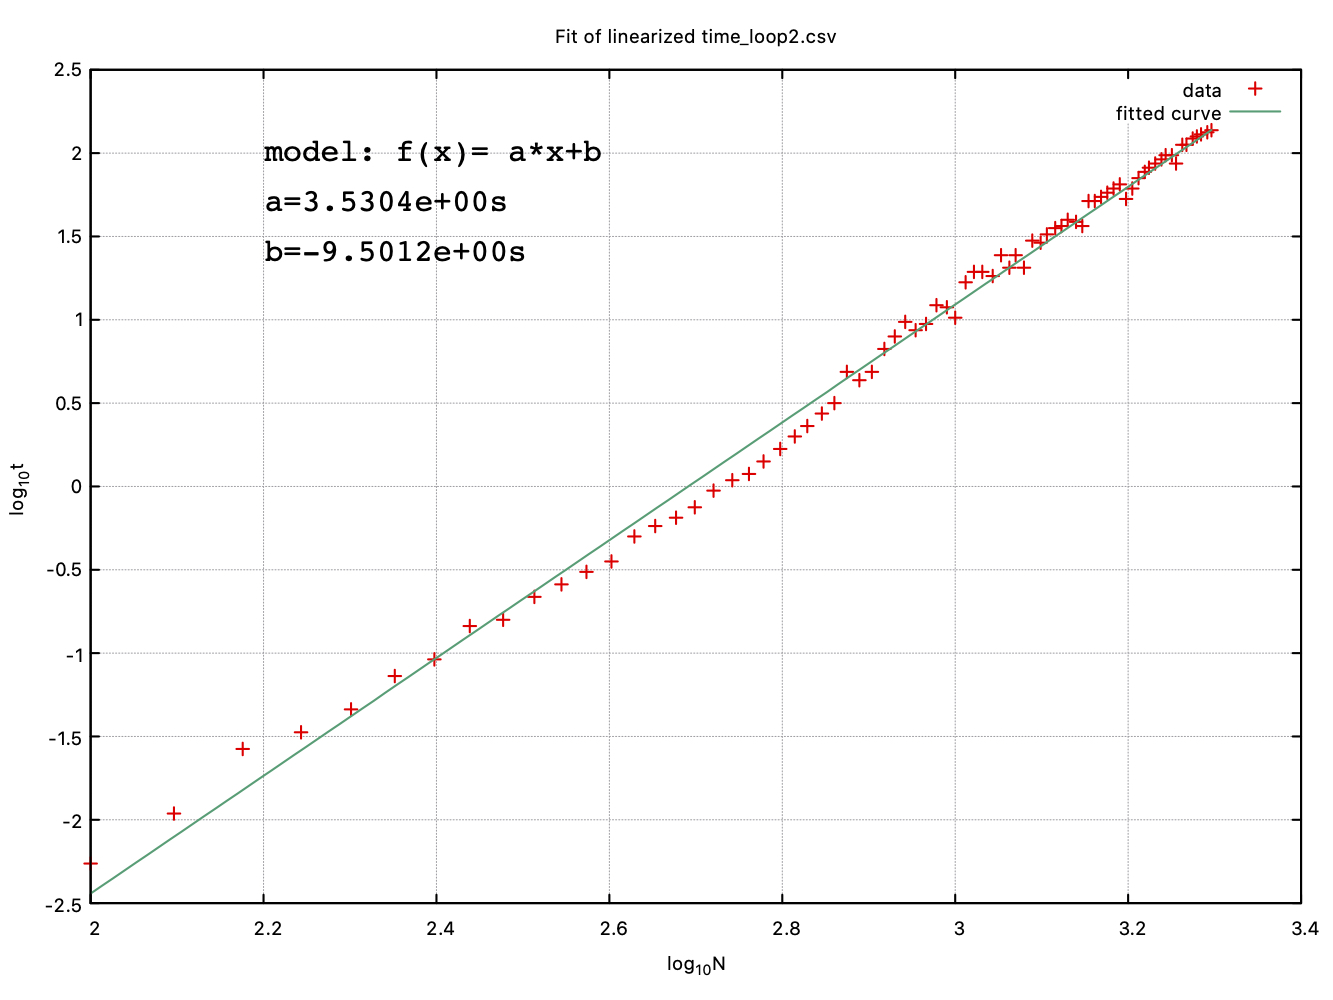
\includegraphics[width=.32\textwidth]{time_loop2_lin}\hfill
    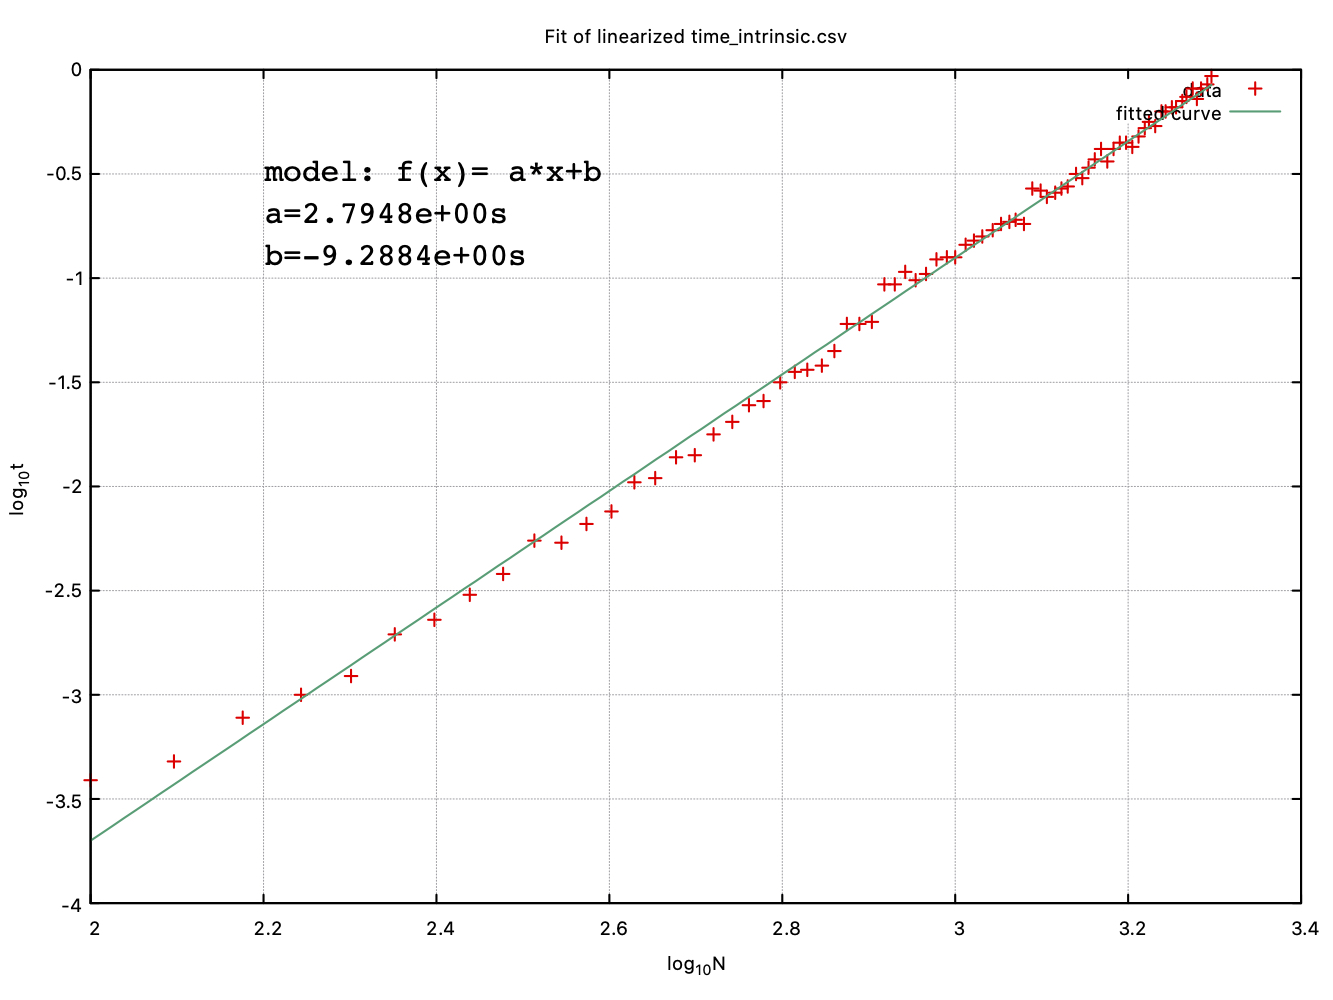
\includegraphics[width=.32\textwidth]{time_intrinsic_lin}
    \caption{Some images}\label{fig:foobar}
\end{figure}

\section{Self-evaluation}
I think the main objectives of the exercises are reached. Probably, I don't have produced the most fancy graphs with Gnuplot but it's the first approach for me.



\end{document}
